\documentclass[10pt,twocolumn,letterpaper]{article}

\usepackage{cvpr}
\usepackage{times}
\usepackage{epsfig}
\usepackage{graphicx}
\usepackage{amsmath}
\usepackage{amssymb}
\usepackage{booktabs}
\usepackage{xcolor}

\usepackage[breaklinks=true,bookmarks=false]{hyperref}

\cvprfinalcopy % camera-ready (non-anonymous) version

\def\cvprPaperID{****}
\def\httilde{\mbox{\tt\raisebox{-.5ex}{\symbol{126}}}}

% Draft marker for anything not yet computed. Remove before submission.
\newcommand{\tbd}[1]{\textcolor{red}{[TBD: #1]}}

\graphicspath{{figures/}{../figures/explore/}{../figures/results/}}

\ifcvprfinal\pagestyle{empty}\fi
\begin{document}

%%%%%%%%% TITLE
\title{Physics-Guided Temporal Transformer for Aviation\\Effective Dose-Rate Estimation}

\author{Sanjib K C\\
{\tt\small skc3@gsu.edu}
}

\maketitle
\thispagestyle{empty}

%%%%%%%%% ABSTRACT
\begin{abstract}
Aircrew and passengers are exposed to cosmic radiation at cruising altitude,
but the dose rate is measured on only a few flights, so operational estimates
rely on physics models. Using 92,415 in-flight measurements, we show that the
physics model NAIRAS V3 underpredicts 89\% of observations above
15~$\mu$Sv/h and cannot tell from its own estimate which flights will receive
high doses. We train a Transformer to learn a correction to NAIRAS from the
aircraft's location and the recent history of solar and geomagnetic
conditions, compare it with static machine-learning and convolutional
baselines, and use attention and attribution to identify which conditions and
time lags drive the correction. Over 18 runs on unseen flights, temporal
networks reduce error by 9.5\% relative to NAIRAS, significantly more than a
network without history and on par with the best static model, and a
high-dose-weighted Transformer reduces error above 15~$\mu$Sv/h by 19\% at no
overall cost.
\end{abstract}

%%%%%%%%% BODY TEXT
\section{Introduction}
\label{sec:intro}

Galactic cosmic rays and solar energetic particles produce showers of
secondary radiation in the atmosphere, and the resulting dose rate at
cruising altitude is many times higher than at the ground. Aircrew are
therefore among the most radiation-exposed occupational groups. Direct
measurements, such as those from the Automated Radiation Measurements for
Aerospace Safety (ARMAS) system~\cite{tobiska2016}, exist for only a small
number of flights, so routine dose estimates depend on physics-based models
such as NAIRAS~\cite{mertens2013}.

The high-dose regime is where these models fail and where accuracy matters
most. On the ARMAS dataset~\cite{sadykov2026}, NAIRAS V3 has an RMSE of
4.05~$\mu$Sv/h overall but 6.86~$\mu$Sv/h when the measured dose exceeds
15~$\mu$Sv/h, and it underpredicts 89\% of those observations
(Sec.~\ref{sec:eda}). The failure is not a simple offset: grouped by its own
estimate, NAIRAS is nearly unbiased, yet its errors in each group range widely
in both directions (Fig.~\ref{fig:nairas}d). In other words, NAIRAS cannot
identify \emph{which} flights will receive high doses.

Static machine-learning corrections~\cite{kc2025} reduce this error using the
geospace conditions at the observation time, but they treat each observation
independently. The dose, however, depends on interacting factors that evolve
in time: altitude, the geomagnetic shielding of the aircraft's location, the
phase of the solar cycle, and short-lived disturbances such as geomagnetic
storms. We hypothesize that the recent history of these conditions carries
information about the dose that a single snapshot misses.

We address these gaps with a physics-guided temporal model. A Transformer
encoder~\cite{vaswani2017} reads the recent history of 35 solar,
interplanetary, and geomagnetic variables and predicts the \emph{residual}
between ARMAS and NAIRAS, so that the physics model supplies the baseline and
the network supplies what it misses. Our contributions are:
(i) an exploratory analysis showing where and why NAIRAS fails;
(ii) a residual Transformer compared with NAIRAS, a prior static model, and
MLP, 1D-CNN, CNN--MLP, and TCN baselines;
(iii) a comparison of a 1-hour (5-minute cadence) and a 24-hour (hourly
cadence) history to test how far back space weather matters;
(iv) an imbalance-aware loss for the rare high-dose regime; and
(v) attention and integrated-gradient analysis of lead--lag effects.

\section{Related Work}
\label{sec:related}

\textbf{Physics-based aviation dose models.}
NAIRAS~\cite{mertens2013} and CARI-7~\cite{copeland2017} propagate cosmic-ray
spectra through the geomagnetic field and atmosphere to compute dose at any
location and altitude. They require no flight measurements, but their
simplified inputs cause systematic biases that measurement campaigns such as
ARMAS~\cite{tobiska2016} have exposed. We keep NAIRAS V3 as the baseline and
learn its error rather than replacing it.

\textbf{Machine learning for space weather and aviation dose.}
Camporeale~\cite{camporeale2019} reviews machine-learning nowcasting in space
weather and highlights scarce data and rare extreme events. Sadykov
\etal~\cite{sadykov2026} released machine-learning-ready datasets that align
ARMAS and NAIRAS with flight position, neutron-monitor counts, solar-wind
parameters, particle fluxes, and geomagnetic indices. Our earlier
work~\cite{kc2025} used the current-time conditions to correct NAIRAS; it
serves as our static baseline. Wang \etal~\cite{wang2024} train a neural
network to reproduce simulated dose rapidly, whereas we correct a physics model
against measurements. Sequence models fed with solar-wind history already
forecast geomagnetic indices, using LSTMs~\cite{gruet2018}, convolutional and
recurrent layers~\cite{collado2021}, and Transformers~\cite{abduallah2024}; we
apply the same idea to the dose itself.

\textbf{Physics-guided learning.}
Theory-guided data science~\cite{karpatne2017} and later
reviews~\cite{willard2022,reichstein2019} argue that combining physical models
with learning improves generalization over either alone. Physics-informed
networks~\cite{raissi2019,karniadakis2021} place physics in the loss; we
instead place it in the output, learning the residual of NAIRAS, and test this
against direct prediction with otherwise identical networks.

\textbf{Temporal models and imbalanced targets.}
Temporal convolutional networks~\cite{bai2018} and
Transformers~\cite{vaswani2017,lim2021} model multivariate sequences, and
attention weights can expose which time steps a prediction uses, although
whether attention explains a prediction is debated~\cite{jain2019,wiegreffe2019},
so we compare it with integrated gradients~\cite{sundararajan2017}. Unlike
long-horizon forecasting, our sequences are short and strongly
autocorrelated, so whether attention helps is an empirical question. For
skewed targets, Yang \etal~\cite{yang2021} show that standard losses
underperform in sparse target regions, and Ribeiro and
Moniz~\cite{ribeiro2020} propose metrics for extreme values; we use a threshold-weighted Huber
loss~\cite{huber1964} because the high-dose threshold is defined
operationally.

\section{Model and Method}
\label{sec:method}

\subsection{Dataset}
\label{sec:data}
The dataset~\cite{sadykov2026} contains 92,415 ARMAS observations from
2013--2023, split by flight into three partitions
(Table~\ref{tab:partitions}) so that no flight contributes to more than one.
Each observation has the measured effective dose rate $A$ (the target), the
NAIRAS V3 estimate $N$, and 43 input features of two kinds
(Table~\ref{tab:features}). The 8 \emph{static} features describe the
aircraft's position and geomagnetic shielding at the observation time and
have a single value per observation. The 35 \emph{temporal} features describe
the solar, interplanetary, and geomagnetic environment and are given as a
history: 12 steps at 5-minute cadence covering the preceding 55~min, or, for
the same observations, 24 steps at hourly cadence covering the preceding
23~h. The last step of each history is the observation time, so the current
value of every temporal feature is also available. The vehicle identifier is
excluded from all inputs.

\begin{table}[t]
\caption{Input features. Static features have one value per observation;
temporal features have a history of $T=12$ five-minute steps or $T=24$ hourly
steps ending at the observation time. Kp is a quasi-logarithmic 3-hourly
index of global geomagnetic disturbance, and ap is its linear equivalent, so
both are constant within each 3-hour interval.}
\label{tab:features}
\centering\small
\begin{tabular}{p{0.24\linewidth}p{0.62\linewidth}}\toprule
Group (count) & Features \\ \midrule
\multicolumn{2}{l}{\emph{Static: shape $8$}} \\
Position (4) & latitude, longitude, barometric and GPS altitude \\
Geomagnetic (4) & geomagnetic latitude and longitude, cutoff rigidity $R_c$, L-shell \\ \midrule
\multicolumn{2}{l}{\emph{Temporal: shape $T\times35$}} \\
Neutron monitors (4) & Newark, Oulu, Thule, South Pole count rates \\
Solar X-rays (2) & short- and long-wavelength flux \\
Energetic particles (7) & protons $>$1, 5, 10, 30, 50, 100~MeV; electrons \\
Solar wind (11) & $|B|$, $B_x$, $B_y$, $B_z$, speed and components, density, temperature, pressure \\
Geomagnetic indices (3) & Kp, ap, Dst \\
Solar activity (8) & sunspot number, F10.7, and Wilcox Solar Observatory north, south, and average polar field, each raw and 20~nHz low-pass filtered \\ \bottomrule
\end{tabular}
\end{table}

\begin{table}[t]
\caption{Flight-separated partitions. $A>15$ counts observations whose
measured dose rate exceeds 15~$\mu$Sv/h. NAIRAS RMSE (in $\mu$Sv/h) is
computed against ARMAS over all observations and over the high-dose subset.
The partitions have similar high-dose fractions and NAIRAS errors, so any of
them can serve as a fair test set.}
\label{tab:partitions}
\centering\small
\begin{tabular}{lrrrr}\toprule
 & & & \multicolumn{2}{c}{NAIRAS RMSE} \\ \cmidrule(l){4-5}
Partition & Rows & $A>15$ & All & $A>15$ \\ \midrule
P1 & 32,369 & 5,324 (16.4\%) & 4.08 & 7.16 \\
P2 & 30,752 & 4,983 (16.2\%) & 4.07 & 6.87 \\
P3 & 29,294 & 4,947 (16.9\%) & 3.99 & 6.50 \\ \midrule
All & 92,415 & 15,254 (16.5\%) & 4.05 & 6.86 \\ \bottomrule
\end{tabular}
\end{table}

\subsection{Exploratory Analysis: Where NAIRAS Fails}
\label{sec:eda}

Fig.~\ref{fig:nairas}a plots NAIRAS against ARMAS. Above 15~$\mu$Sv/h the
cloud is nearly flat: the measured dose reaches 40~$\mu$Sv/h, while NAIRAS
stays near 10--15~$\mu$Sv/h. Grouping the error $r=A-N$ by the measured dose
(Fig.~\ref{fig:nairas}c) shows a median error that grows from negative values to
$+17$~$\mu$Sv/h, whereas grouping by the NAIRAS estimate
(Fig.~\ref{fig:nairas}d) gives a median near zero with an interquartile range
of roughly 5~$\mu$Sv/h that straddles zero. The two views differ because
selecting by the measured value also selects measurements that happened to be
high. Together they show that NAIRAS is approximately unbiased for a given
estimate but cannot distinguish high-dose flights from ordinary ones; the
missing information must come from other inputs.

\begin{figure}[t]
\centering
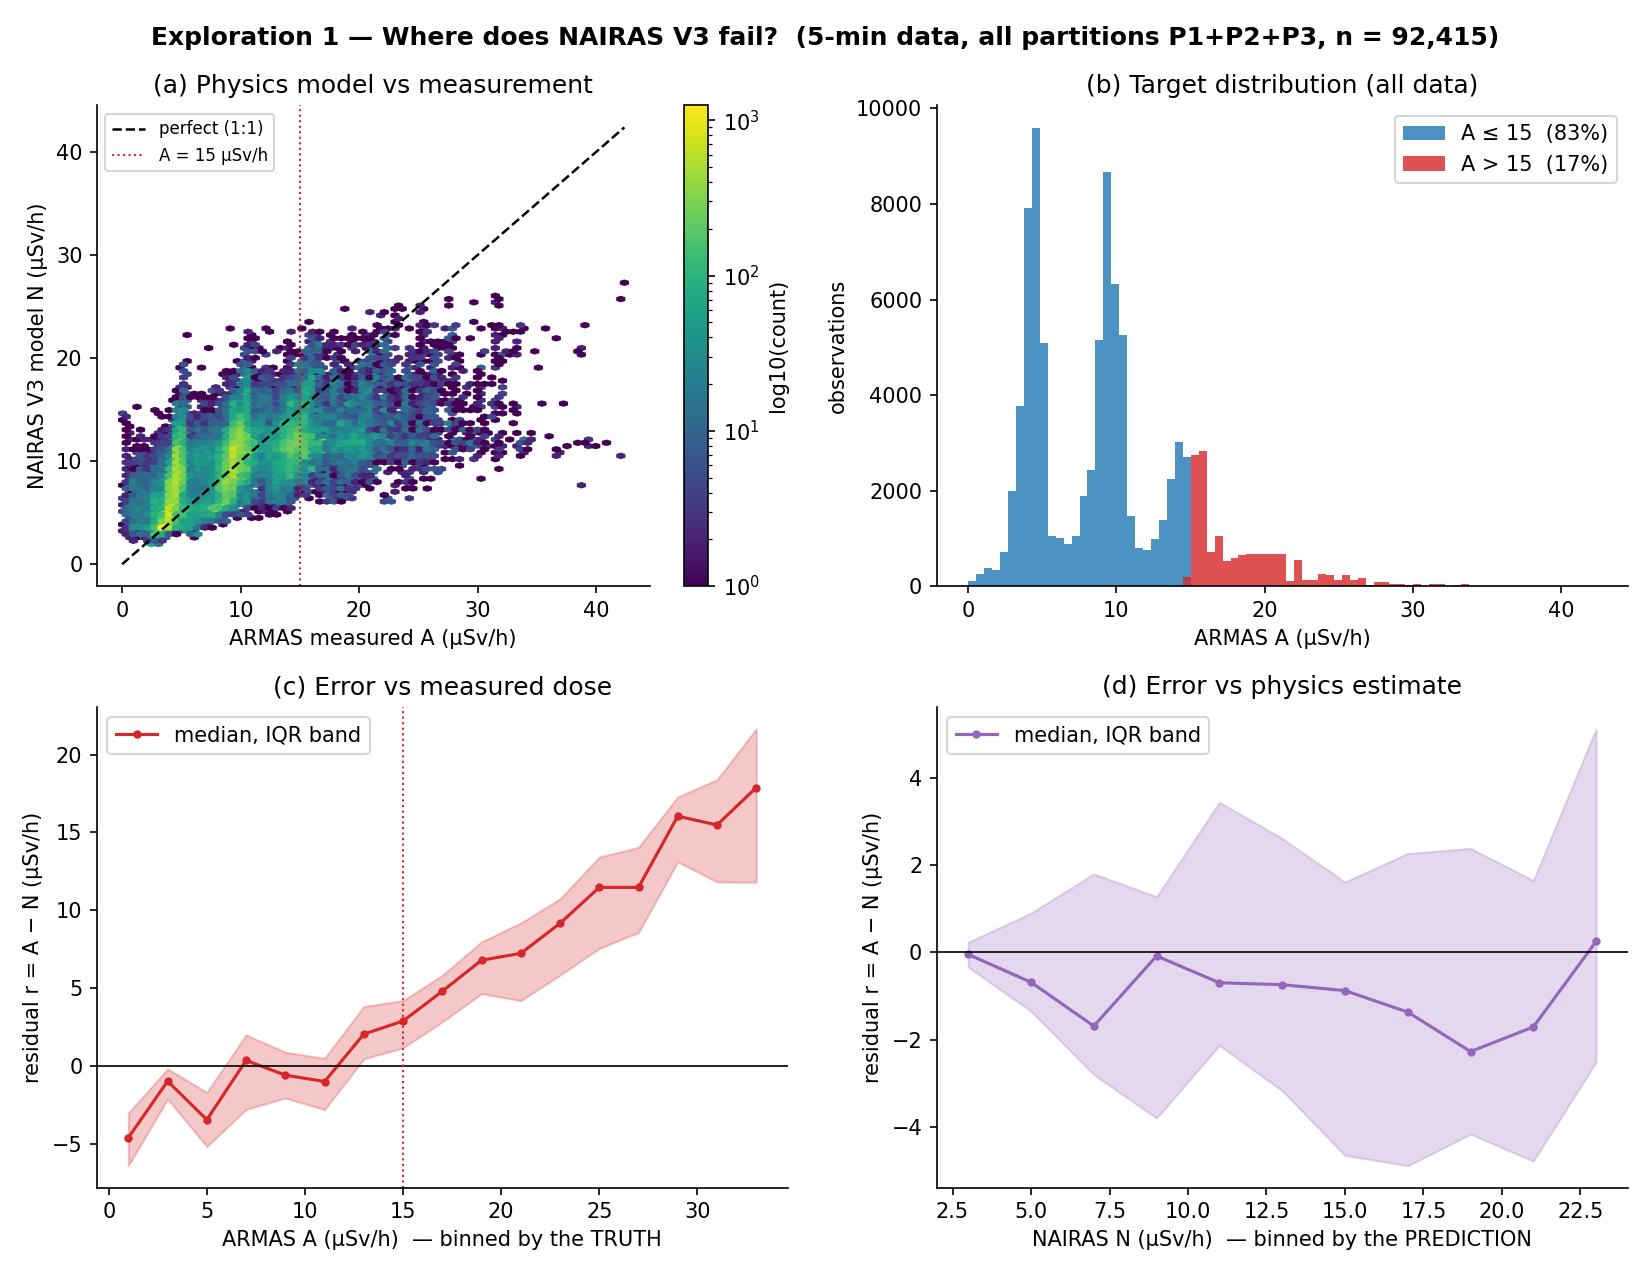
\includegraphics[width=\linewidth]{e01_where_nairas_fails.png}
\caption{NAIRAS V3 against ARMAS for all 92,415 observations.
(a) NAIRAS versus measured dose; the dashed line is perfect agreement.
(b) Distribution of the measured dose; 16.5\% exceeds 15~$\mu$Sv/h.
(c, d) Error $A-N$ grouped in 2~$\mu$Sv/h bins of the measured dose (c) and of
the NAIRAS estimate (d); lines are medians and bands span the 25th--75th
percentiles. NAIRAS is nearly unbiased for a given estimate (d) but misses the
highest measured doses (a, c).}
\label{fig:nairas}
\end{figure}

\textbf{Geomagnetic shielding and altitude interact.}
The distribution of measured dose has peaks near 4.5, 9.5, and
15~$\mu$Sv/h (Fig.~\ref{fig:nairas}b) that correspond to different
geomagnetic shielding: the median cutoff rigidity falls from 4.9 to 2.4 to
1.8~GV across the three peaks at similar altitude. Fig.~\ref{fig:map} shows the
flight tracks. Above 15~$\mu$Sv/h, 36\% of observations with $R_c<1$~GV
qualify, but none with $R_c>10$~GV. Flights near Hawaii cruise highest
(median 13.6~km) yet record the lowest dose (median 3.8~$\mu$Sv/h) because
the shielding there is strong ($R_c\approx12$~GV). The dose therefore depends
on interactions between inputs, which motivates a nonlinear model. Map (c)
shows that high and low NAIRAS errors occur in the same regions, so location
alone cannot explain the error.

\begin{figure*}[t]
\centering
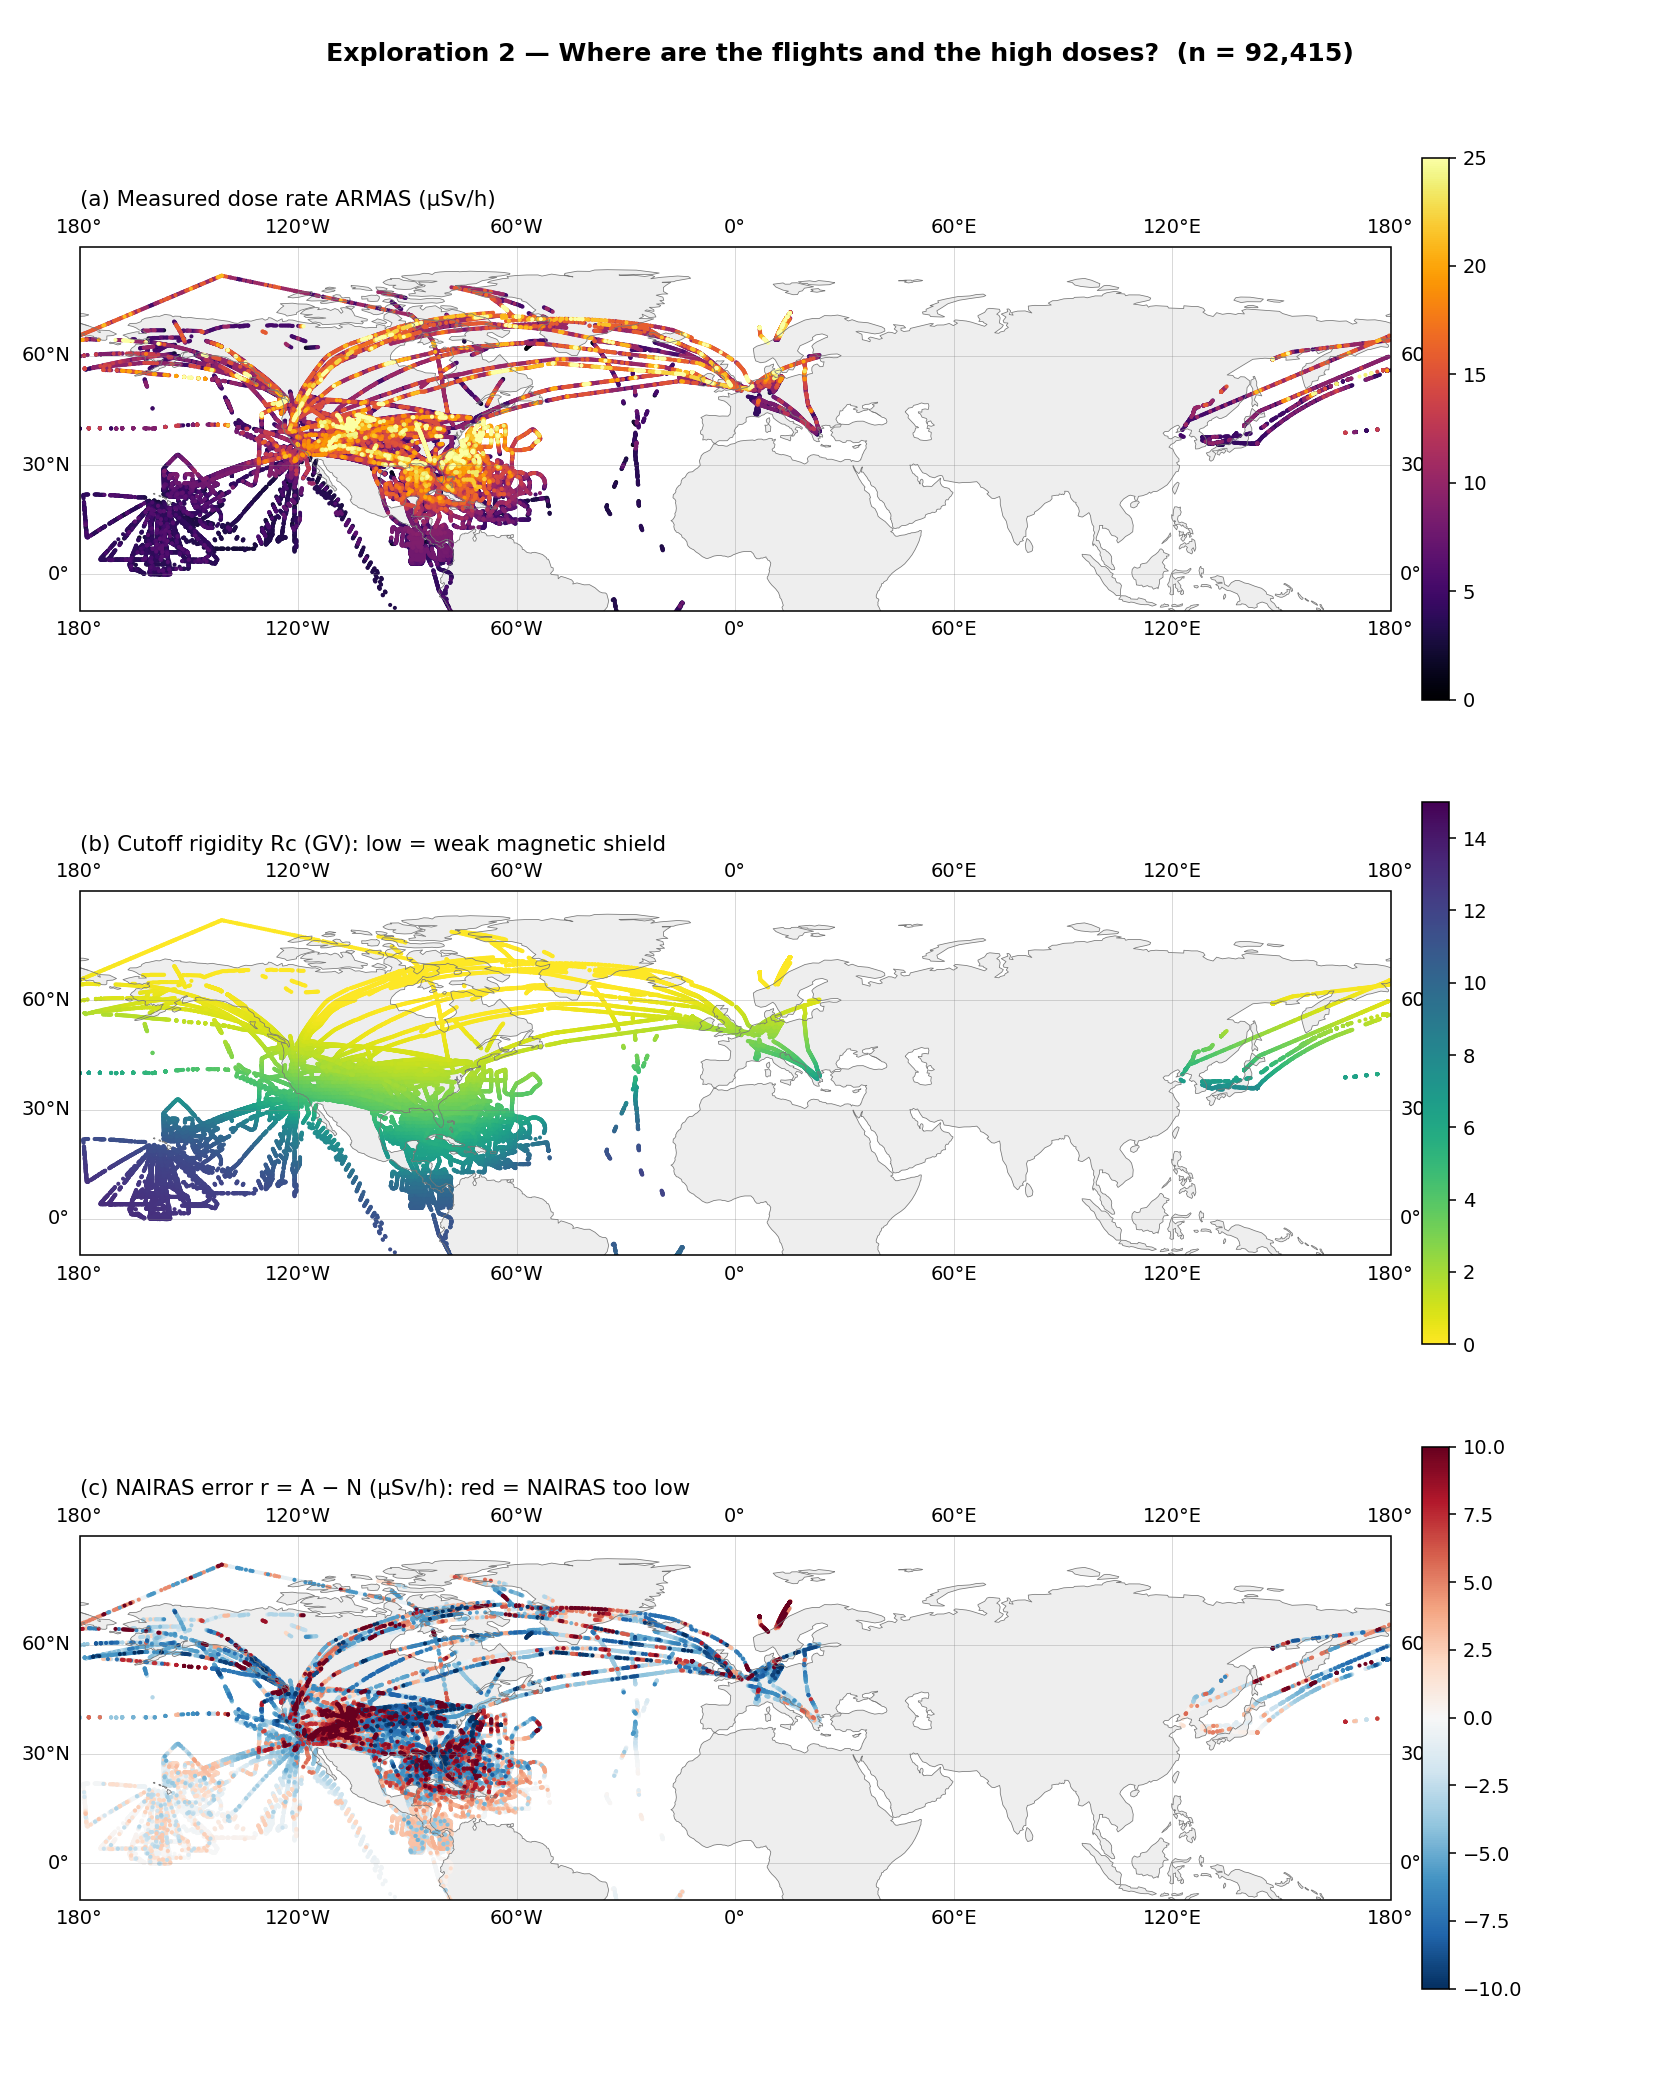
\includegraphics[width=0.9\linewidth]{e02_flight_map.png}
\caption{Flight tracks of all observations colored by (a) measured dose rate,
(b) geomagnetic cutoff rigidity $R_c$ (low values mean weak magnetic
shielding), and (c) NAIRAS error $A-N$ (red: NAIRAS too low). High doses
concentrate where shielding is weak, but positive and negative NAIRAS errors
are interleaved in the same regions, so the error depends on more than
location.}
\label{fig:map}
\end{figure*}

\textbf{Solar modulation.}
Over the solar cycle, sunspot number and Oulu neutron-monitor counts are
anticorrelated ($r=-0.76$ across flight-days), as expected from solar
modulation of galactic cosmic rays (Appendix Fig.~\ref{fig:solar}). To
remove the effect of location, we keep only observations with matched
shielding and altitude ($R_c<1$~GV, 10.5--12~km) and only days with at least
10 such observations, which leaves 43 flight-days. On these days NAIRAS follows the neutron-monitor counts closely
($r=0.81$) and falls by 3.1~$\mu$Sv/h per 100 sunspots, the expected
solar-modulation response, whereas ARMAS shows almost no dependence
($r=-0.10$ with neutron-monitor counts; 0.06~$\mu$Sv/h per 100 sunspots).
With only 43 matched flight-days we report this difference without
attributing it to either the model or the instrument. An active Sun can also raise the dose through solar energetic particle
(SEP) events, most strongly in ground-level enhancements (GLEs). The dataset
contains no such exposure: during the September 2017 SEP event the aircraft
flew at $R_c=3$--10~GV, where the geomagnetic field blocks solar protons, and
the only polar flight during an SEP alert (March 2023) coincided with a weak
event with negligible $>$100~MeV flux. The models therefore learn
galactic-cosmic-ray conditions only.

\textbf{Measurement characteristics.}
In 56\% of consecutive records the ARMAS value is unchanged, so neighboring
records are not independent. A random row-level split would place nearly
identical records in training and test sets; we therefore keep the
flight-separated partitions throughout. These repeats, and the conversion
from silicon absorbed dose to effective dose, also imply an irreducible
measurement noise floor.

\textbf{Information in the history.}
Appendix Fig.~\ref{fig:temporal}a measures how much each variable changes
inside its window. Within one hour, 16 of the 35 variables are effectively
constant, including the Kp and Ap indices (reported every three hours), the
daily solar indices, and X-ray fluxes, so a 1-hour history can add little
for them. Over 24 hours, the solar-wind magnetic field and velocity, Kp, Dst,
and solar-wind pressure change by one to two standard deviations.
Lead--lag maps of the Spearman correlation between the NAIRAS error and each
variable at each lag (Appendix Fig.~\ref{fig:temporal}b,c) show that the
strongest associations come from neutron-monitor counts ($|\rho|\approx0.17$)
and are nearly constant across lags. In contrast, Kp and Ap are more strongly
associated with the error about 15~h before the observation
($\rho\approx0.12$) than at the observation time ($\rho\approx0.04$). These
associations are weak individually, but they suggest that geomagnetic
activity acts on the error with a delay of hours, which only a 24-hour
history can represent; Sec.~\ref{sec:attention} tests whether the
networks use it.

\subsection{Physics-Guided Residual Formulation}
Let $X_i\in\mathbb{R}^{T\times35}$ be the environmental history ($T=12$ or
24), $s_i\in\mathbb{R}^{8}$ the current flight and geomagnetic variables, and
$N_i$ the NAIRAS estimate. The residual model learns the NAIRAS error and
reconstructs the dose as
\begin{equation}
r_i = A_i - N_i, \qquad
\hat{A}_i = N_i + f_\theta(X_i, s_i, N_i),
\label{eq:residual}
\end{equation}
where $f_\theta$ is a network with parameters $\theta$. Direct models predict
$A_i$ without $N_i$.

\subsection{Temporal Transformer}
Each time step is projected to a $d$-dimensional embedding with a positional
encoding, and self-attention lets every step weigh every other,
\begin{equation}
\mathrm{Attn}(Q,K,V)=\mathrm{softmax}\!\left(\frac{QK^\top}{\sqrt{d}}\right)V,
\label{eq:attention}
\end{equation}
where $Q$, $K$, and $V$ are learned linear projections of the embeddings.
Attention (Eq.~\eqref{eq:attention}) operates on tokens. Each hour (or 5-minute step) is one token: its 35 standardized values are
projected to $d=16$ dimensions and given a learned position embedding. A
learned summary token is prepended, two pre-normalized encoder blocks with
four heads are applied, and the summary token's output is concatenated with
an embedding of the eight static variables and $N_i$ before a small output
network predicts $r_i$ (8,993 parameters). Heavy-tailed X-ray and particle
fluxes are log-transformed before standardization.

\subsection{Baselines}
The baselines form a ladder in which each model adds one idea, so that each
gain can be attributed. They are NAIRAS V3; the static models of K C
\etal~\cite{kc2025}, quoted from that study; a current-time MLP (43 inputs,
128 and 64 hidden units, 14,081 parameters); a Flat MLP that receives the
whole history as one 840-value vector (56,513 parameters); a hybrid CNN--MLP
with two convolutions over time (7,025); a causal dilated TCN~\cite{bai2018}
(10,369); and a direct Transformer that predicts $A$ without NAIRAS. Every
model except the direct ones learns the residual of Eq.~\eqref{eq:residual}. On the static version of the dataset, the best static model of
\cite{kc2025}, XGBoost, reached a test RMSE of $3.671\pm0.061$~$\mu$Sv/h
against $4.045\pm0.087$ for NAIRAS, a 9.3\% reduction, with random forest
($3.725\pm0.067$) and LASSO ($3.853\pm0.077$) behind it (mean $\pm$ standard
deviation over partition rotations). That study did not report high-dose
errors, which we add here.

\subsection{Training Objective}
All networks minimize a weighted Huber loss~\cite{huber1964},
\begin{equation}
\mathcal{L}(\theta) = \frac{1}{n}\sum_{i=1}^{n} w_i\,
\ell_\delta\!\left(y_i - \hat{y}_i\right), \qquad
w_i = \begin{cases} w, & A_i > 15,\\ 1, & \text{otherwise,}\end{cases}
\label{eq:huber}
\end{equation}
where $\ell_\delta$ is the Huber function and $y_i$ the standardized target.
Standard models use $w=1$ and a squared loss; the high-dose variant uses
Eq.~\eqref{eq:huber} with $w=4$. All networks use AdamW (learning rate $10^{-3}$,
$5\times10^{-4}$ for Transformers), weight decay 0.01, dropout 0.3, batch
size 512, gradient clipping at 1.0, and early stopping on validation RMSE
with patience 10. Width, dropout, and weight decay were chosen on the
validation partition of one assignment only (P1 train, P2 validation): a
first pass with 4--8 times more parameters overfit within 2--7 epochs.

\section{Experiments and Results}
\label{sec:experiments}

\subsection{Protocol}
Preprocessing statistics are fitted on the training partition only. Models
and hyperparameters are selected on the validation partition, and the test
partition is evaluated once. The three partitions rotate through the train,
validation, and test roles. We report RMSE, MAE, and $R^2$ overall and for
$A\leq15$ and $A>15$~$\mu$Sv/h, always comparing with NAIRAS on the same
observations. Every model is trained on all six train--validation--test
assignments with three random seeds, and we report the mean and standard
deviation over these 18 runs. Code and instructions to reproduce all results
are available at
\url{https://github.com/thesanjibkc/Deep_learning_project/tree/final-project}.

\subsection{Main Results}
Table~\ref{tab:results} reports test errors over the 18 runs. All networks
beat NAIRAS. Learning the correction is better than learning the dose
directly for both the MLP and the Transformer (paired flight bootstrap,
Table~\ref{tab:ablation}). With the 24-hour history, the TCN, CNN--MLP, and
Transformer reach 3.66--3.67~$\mu$Sv/h, a 9.5\% reduction from NAIRAS that
is significantly better than the current-time MLP (3.737; difference
$-0.07$, 95\% interval $[-0.10,-0.04]$, better in all six assignments).
Averaging the three seeds' predictions lowers the error further to
3.63--3.64. These values match the static XGBoost of~\cite{kc2025} (3.671),
which was evaluated on the static data with its own protocol, so we do not
claim a difference. The Flat MLP, which sees the same history as one vector,
is significantly worse than every structured temporal model (3.91), showing
that how the history is read matters more than having it.

\textbf{High doses.} Above 15~$\mu$Sv/h, the unweighted networks gain only
8--10\%. Weighting high-dose errors four times reduces the high-dose RMSE to
5.56 (1-hour) and 5.66 (24-hour), a 19\% reduction from NAIRAS. The
seed-ensembled weighted Transformer matches the current-time MLP overall
(difference $+0.001$, interval $[-0.04,0.05]$) while lowering high-dose RMSE
by 0.78~$\mu$Sv/h (interval $[-0.89,-0.67]$, all six assignments).

\begin{table}[t]
\caption{Test RMSE ($\mu$Sv/h, lower is better), mean $\pm$ standard
deviation over 18 runs (six train--validation--test assignments of P1--P3
$\times$ three seeds), for all observations and the high-dose subset
$A>15$. Gain is the reduction relative to NAIRAS V3, overall / high dose.
All networks except ``direct'' learn the NAIRAS residual. XGBoost is quoted
from~\cite{kc2025} (static data; high-dose error not reported).}
\label{tab:results}
\centering\small
\setlength{\tabcolsep}{3pt}
\begin{tabular}{lccc}\toprule
Model & All & $A>15$ & Gain (\%) \\ \midrule
NAIRAS V3 & $4.044\pm0.040$ & $6.845\pm0.277$ & -- \\
XGBoost, static~\cite{kc2025} & $3.671\pm0.061$ & -- & 9.3 / -- \\ \midrule
MLP, direct & $3.842\pm0.096$ & $6.627\pm0.203$ & 5.0 / 3.2 \\
MLP & $3.737\pm0.032$ & $6.311\pm0.168$ & 7.6 / 7.8 \\ \midrule
Flat MLP, 24\,h & $3.906\pm0.070$ & $6.731\pm0.264$ & 3.4 / 1.7 \\
CNN--MLP, 24\,h & $3.661\pm0.043$ & $6.212\pm0.261$ & 9.5 / 9.2 \\
TCN, 24\,h & $\mathbf{3.659}\pm0.029$ & $6.173\pm0.193$ & 9.5 / 9.8 \\
Transformer, direct, 24\,h & $3.712\pm0.054$ & $6.417\pm0.230$ & 8.2 / 6.3 \\
Transformer, 24\,h & $3.667\pm0.034$ & $6.309\pm0.148$ & 9.3 / 7.8 \\
Transformer, 1\,h & $3.663\pm0.039$ & $6.261\pm0.125$ & 9.4 / 8.5 \\
Transformer, 1\,h, $w=4$ & $3.762\pm0.080$ & $\mathbf{5.563}\pm0.233$ & 7.0 / 18.7 \\
\bottomrule
\end{tabular}
\end{table}

\begin{table}[t]
\caption{Ablations as paired differences in test RMSE ($\mu$Sv/h; negative
means the first model is better), from a bootstrap that resamples whole
flights within each assignment (1,000 draws), using seed-ensembled
predictions and averaging over the six assignments. Brackets give 95\%
intervals; bold marks intervals that exclude zero.}
\label{tab:ablation}
\centering\small
\setlength{\tabcolsep}{3pt}
\begin{tabular}{lcc}\toprule
Comparison (what changes) & All & $A>15$ \\ \midrule
Residual vs direct MLP (physics baseline) & $\mathbf{-0.07}$ & $\mathbf{-0.30}$ \\
Transformer 24\,h vs MLP (history) & $\mathbf{-0.07}$ & $0.00$ \\
TCN 24\,h vs MLP (history) & $\mathbf{-0.07}$ & $\mathbf{-0.14}$ \\
Transformer vs Flat MLP, 24\,h (structure) & $\mathbf{-0.24}$ & $\mathbf{-0.43}$ \\
Transformer 24\,h vs 1\,h (window) & $+0.01$ & $+0.05$ \\
Weighted vs unweighted Transformer, 24\,h & $\mathbf{+0.07}$ & $\mathbf{-0.67}$ \\
\bottomrule
\end{tabular}
\end{table}

\subsection{1-Hour versus 24-Hour History}
After regularization, the 1-hour and 24-hour histories give the same average
error for every architecture (Table~\ref{tab:results}; Transformer difference
$+0.01$, interval $[-0.01,0.03]$). Before regularization the larger
24-hour models overfit and looked worse or better depending on the
architecture, which shows how easily an uncontrolled comparison misleads.
Because 16 of the 35 variables are constant within an hour and storms are
rare, the extra 23 hours change few predictions, so the average is
unchanged even when individual storm flights benefit
(Sec.~\ref{sec:attention}).

\subsection{What the Correction Uses and What Remains}
\label{sec:attention}
\textbf{Feature importance.} Shuffling one feature group across test flights
(permutation importance, six assignments) raises the Transformer's RMSE most
for altitude ($+0.74$), geomagnetic shielding ($+0.65$), and neutron-monitor
counts ($+0.32$); solar wind, Kp/ap/Dst, and X-ray fluxes each add at most
$0.03$. Shuffling any single hour changes the error by less than
0.03~$\mu$Sv/h, because neighboring hours are redundant.

\textbf{Attention on a storm.} We followed training epoch by epoch for one
flight on 9 September 2017, the morning after a severe geomagnetic storm.
Attention starts uniform and, without any label for storms, concentrates on
the hours 16--18~h before the flight, where Kp peaked at 8.3
(Fig.~\ref{fig:attention}); at the same time the Flat MLP spreads its weight
evenly and begins to memorize after four epochs. This agrees with the
lead--lag analysis of Sec.~\ref{sec:eda}, but it is one flight and one run,
and attention indicates what the model used rather than a physical
cause~\cite{jain2019,wiegreffe2019}. It also does not translate into a strong correction: for that moment NAIRAS
was 7.5~$\mu$Sv/h too low, and scaling the storm in the inputs from 0\% to
150\% changed the networks' predictions by at most 1.1~$\mu$Sv/h.

\textbf{What remains.} The NAIRAS error depends on shielding, altitude, and
storm level; after the Transformer's correction these groupings each explain
less than 1\% of the remaining error variance. About 81\% of the remaining
variance lies within individual flights, from minute to minute, where the
space-weather inputs barely change, and 4--7\% is associated with the
aircraft, which is never an input, against a 3\% chance level. Measurement
variability and instrument differences therefore bound the accuracy reachable
from these inputs.

\begin{figure}[t]
\centering
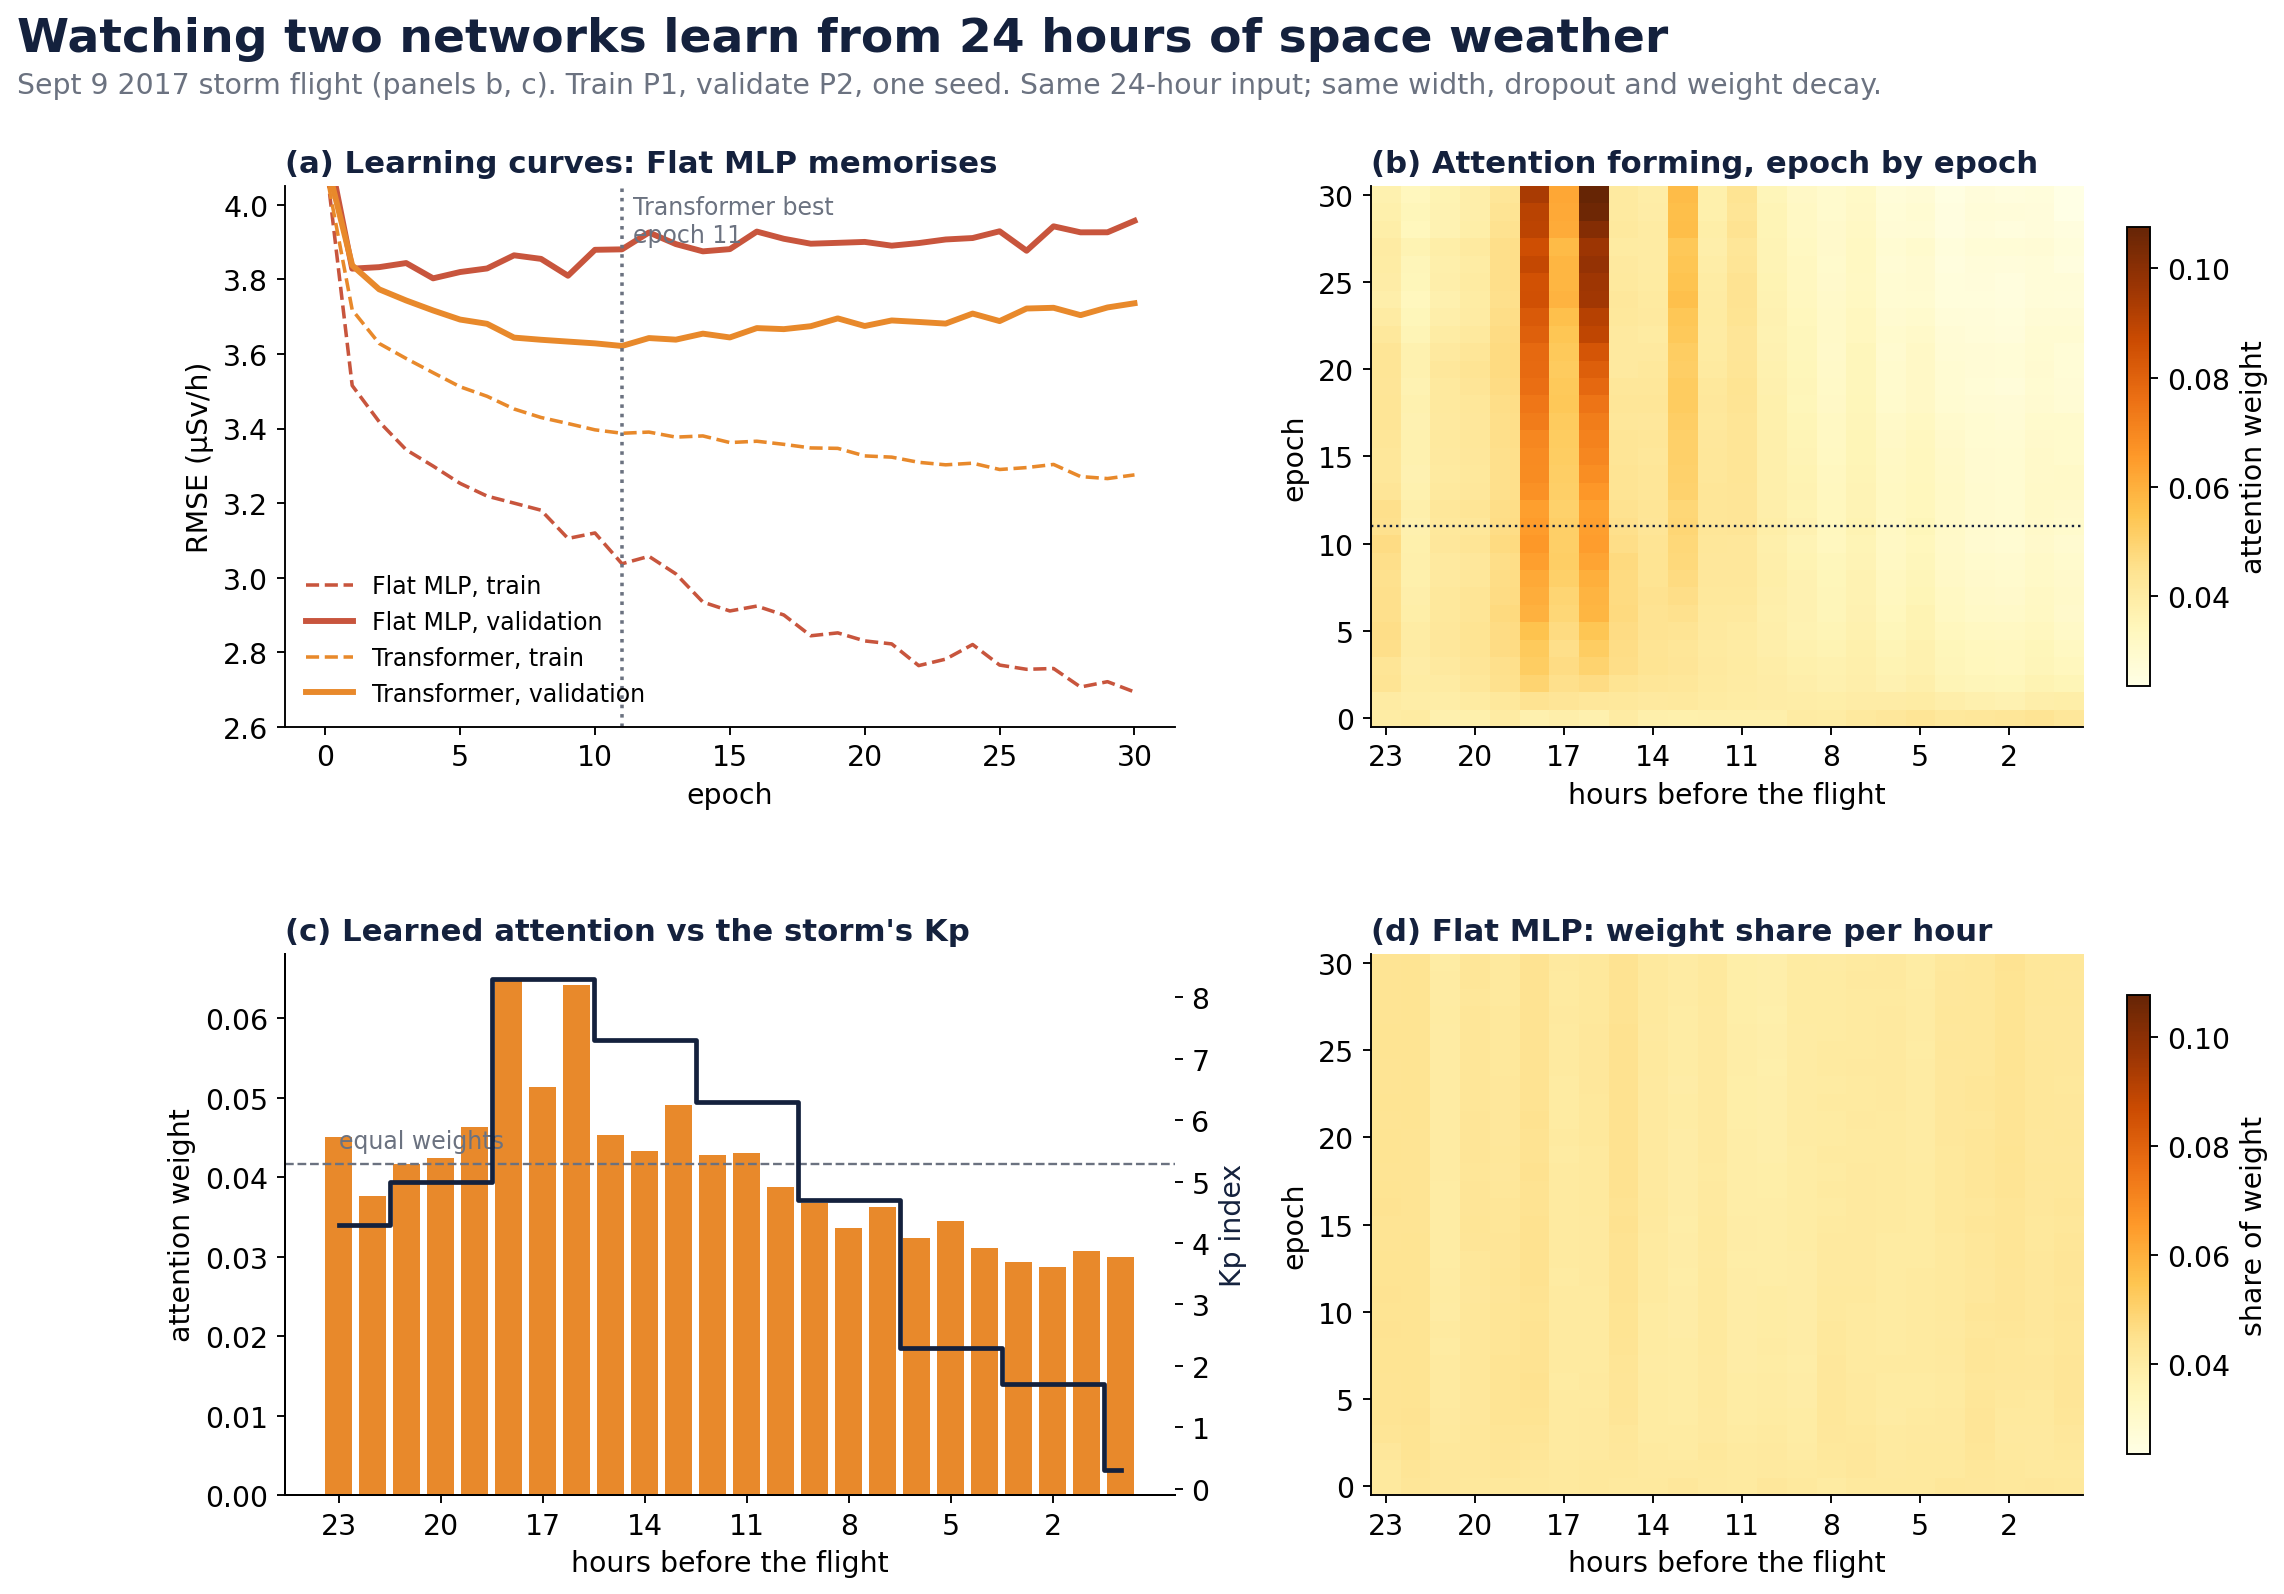
\includegraphics[width=\linewidth]{T1_training_evolution.png}
\caption{Training dynamics with the 24-hour history (P1 train, P2
validation, one seed). (a) Training (dashed) and validation (solid) RMSE:
the Flat MLP memorizes while the Transformer improves until epoch 11.
(b) Transformer attention over the 24 hours for the 9 September 2017 flight
at every epoch. (c) Attention at the best epoch against Kp: the weight
concentrates where Kp peaked at 8.3, 16--18~h before the flight. (d) Flat
MLP first-layer weight share per hour, which stays uniform.}
\label{fig:attention}
\end{figure}

\section{Conclusions}
\label{sec:conclusions}
Three lessons stand out. First, the physics model is the right starting
point: learning NAIRAS's residual was more accurate and three times more
stable than learning the dose directly. Second, recent space-weather history
helps only when it is read with structure and the model is kept small: with
a few hundred training flights, regularized temporal networks beat a
current-time network, while a flat, larger network memorized; a longer
window did not lower the average error, although attention found the
delayed effect of a storm on an individual flight. Third, the objective
matters most for safety: weighting high-dose errors cut the error above
15~$\mu$Sv/h by 19\% relative to NAIRAS without hurting overall accuracy.
The remaining error is mostly within-flight measurement variability and
instrument differences, and no flight in the data was exposed to solar
energetic particles, so the models cover galactic-cosmic-ray conditions only.
Natural next steps are uncertainty estimates from seed ensembles~\cite{lakshminarayanan2017},
per-instrument calibration, and pretraining the history encoder on long
space-weather archives.

\clearpage
\section*{Peer Evaluation}
This is an individual project; all work was performed by the author.

{\small
\bibliographystyle{ieee_fullname}
\bibliography{references}
}

\clearpage
\appendix
\section{Additional Exploratory Figures}

\begin{figure*}[h]
\centering
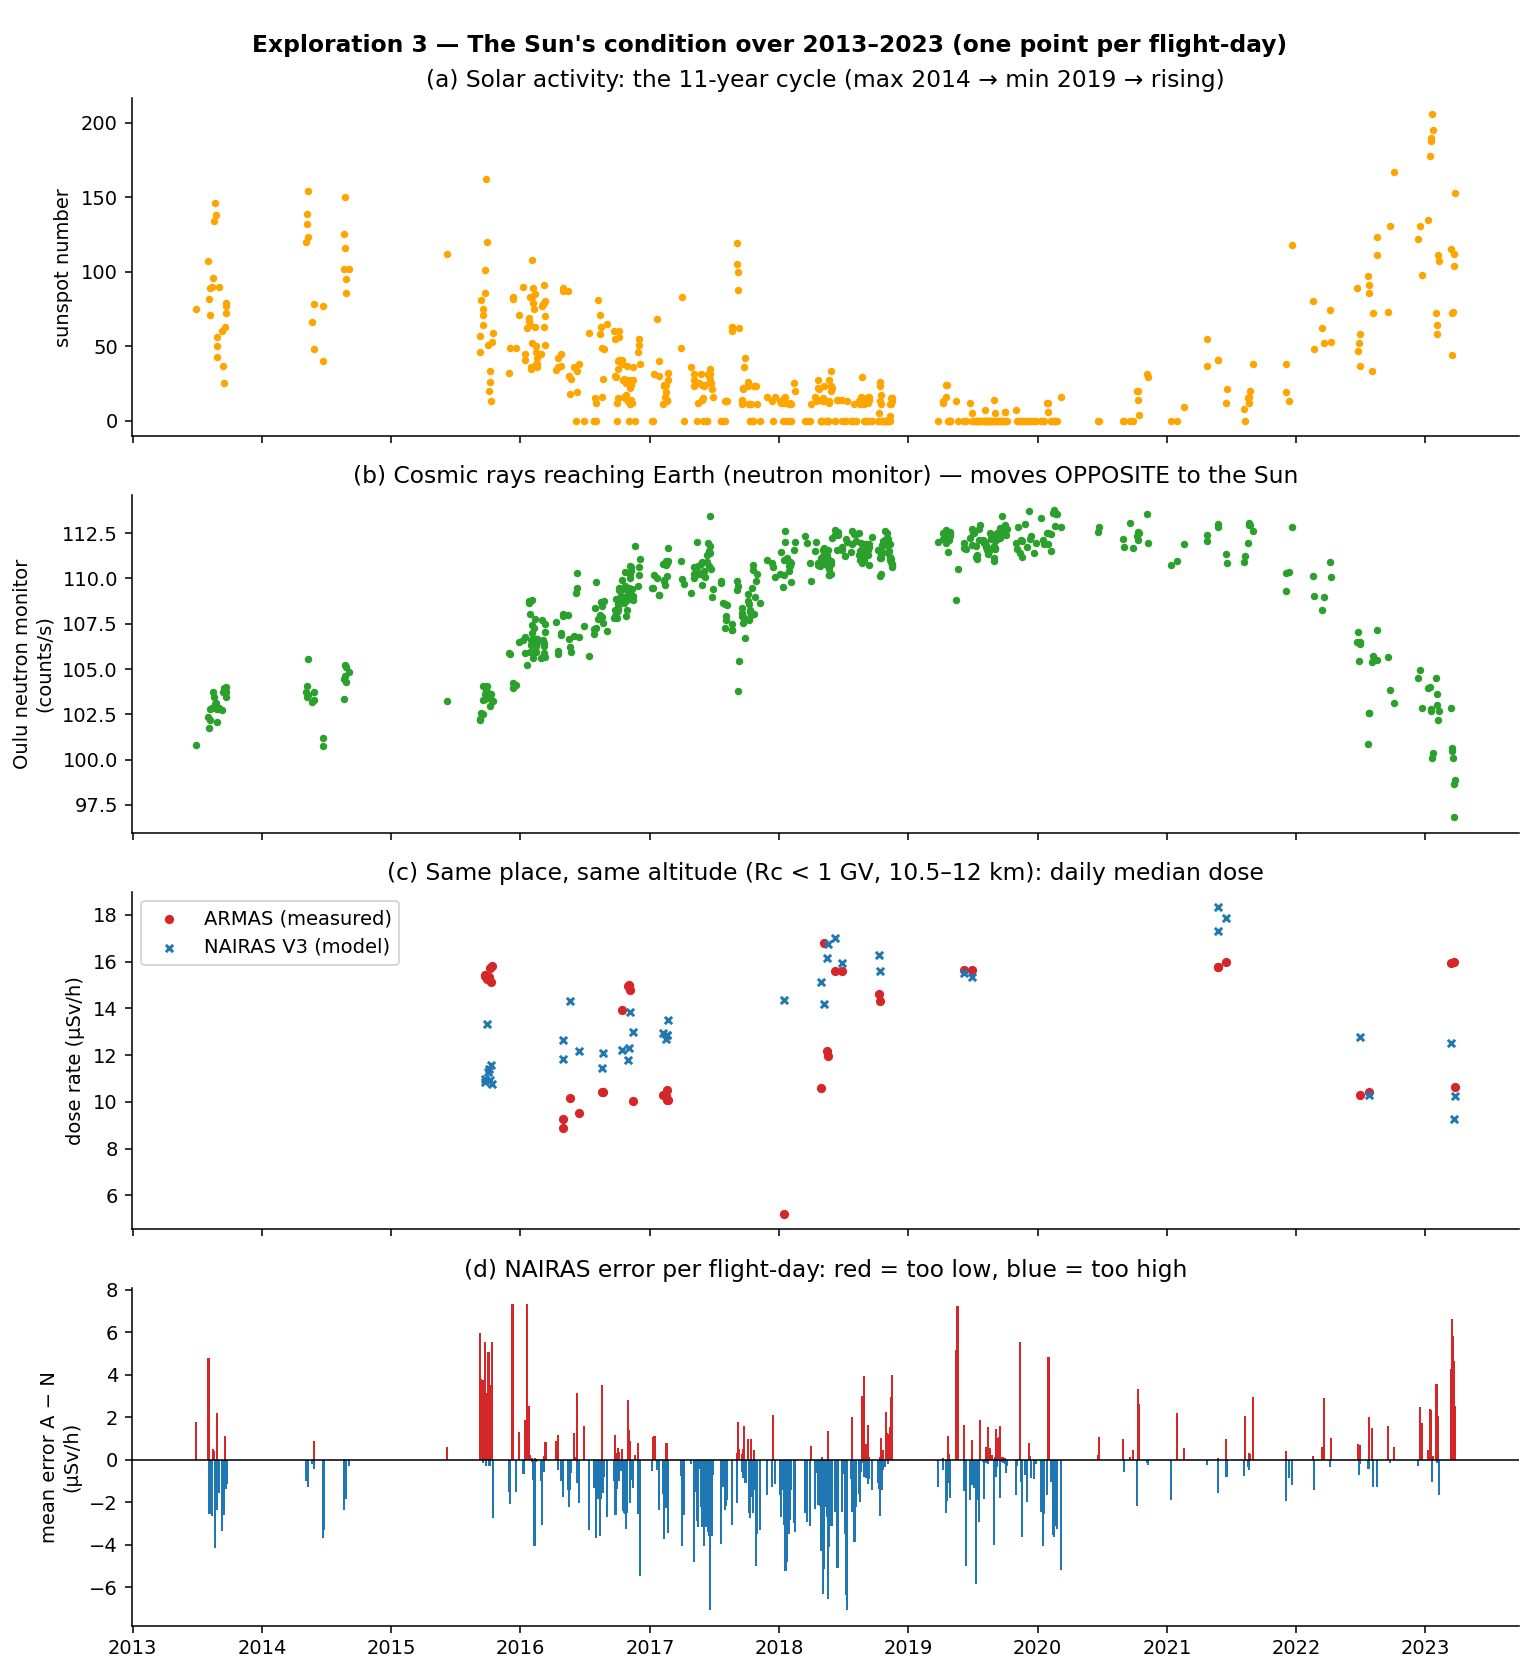
\includegraphics[width=0.85\linewidth]{e03_solar_cycle.png}
\caption{Solar cycle and dose, one point per flight-day. (a) Sunspot number.
(b) Oulu neutron-monitor counts, which move opposite to solar activity.
(c) Daily median ARMAS and NAIRAS for matched conditions ($R_c<1$~GV,
10.5--12~km altitude). (d) Mean NAIRAS error per flight-day (red: NAIRAS too
low; blue: too high).}
\label{fig:solar}
\end{figure*}

\begin{figure*}[h]
\centering
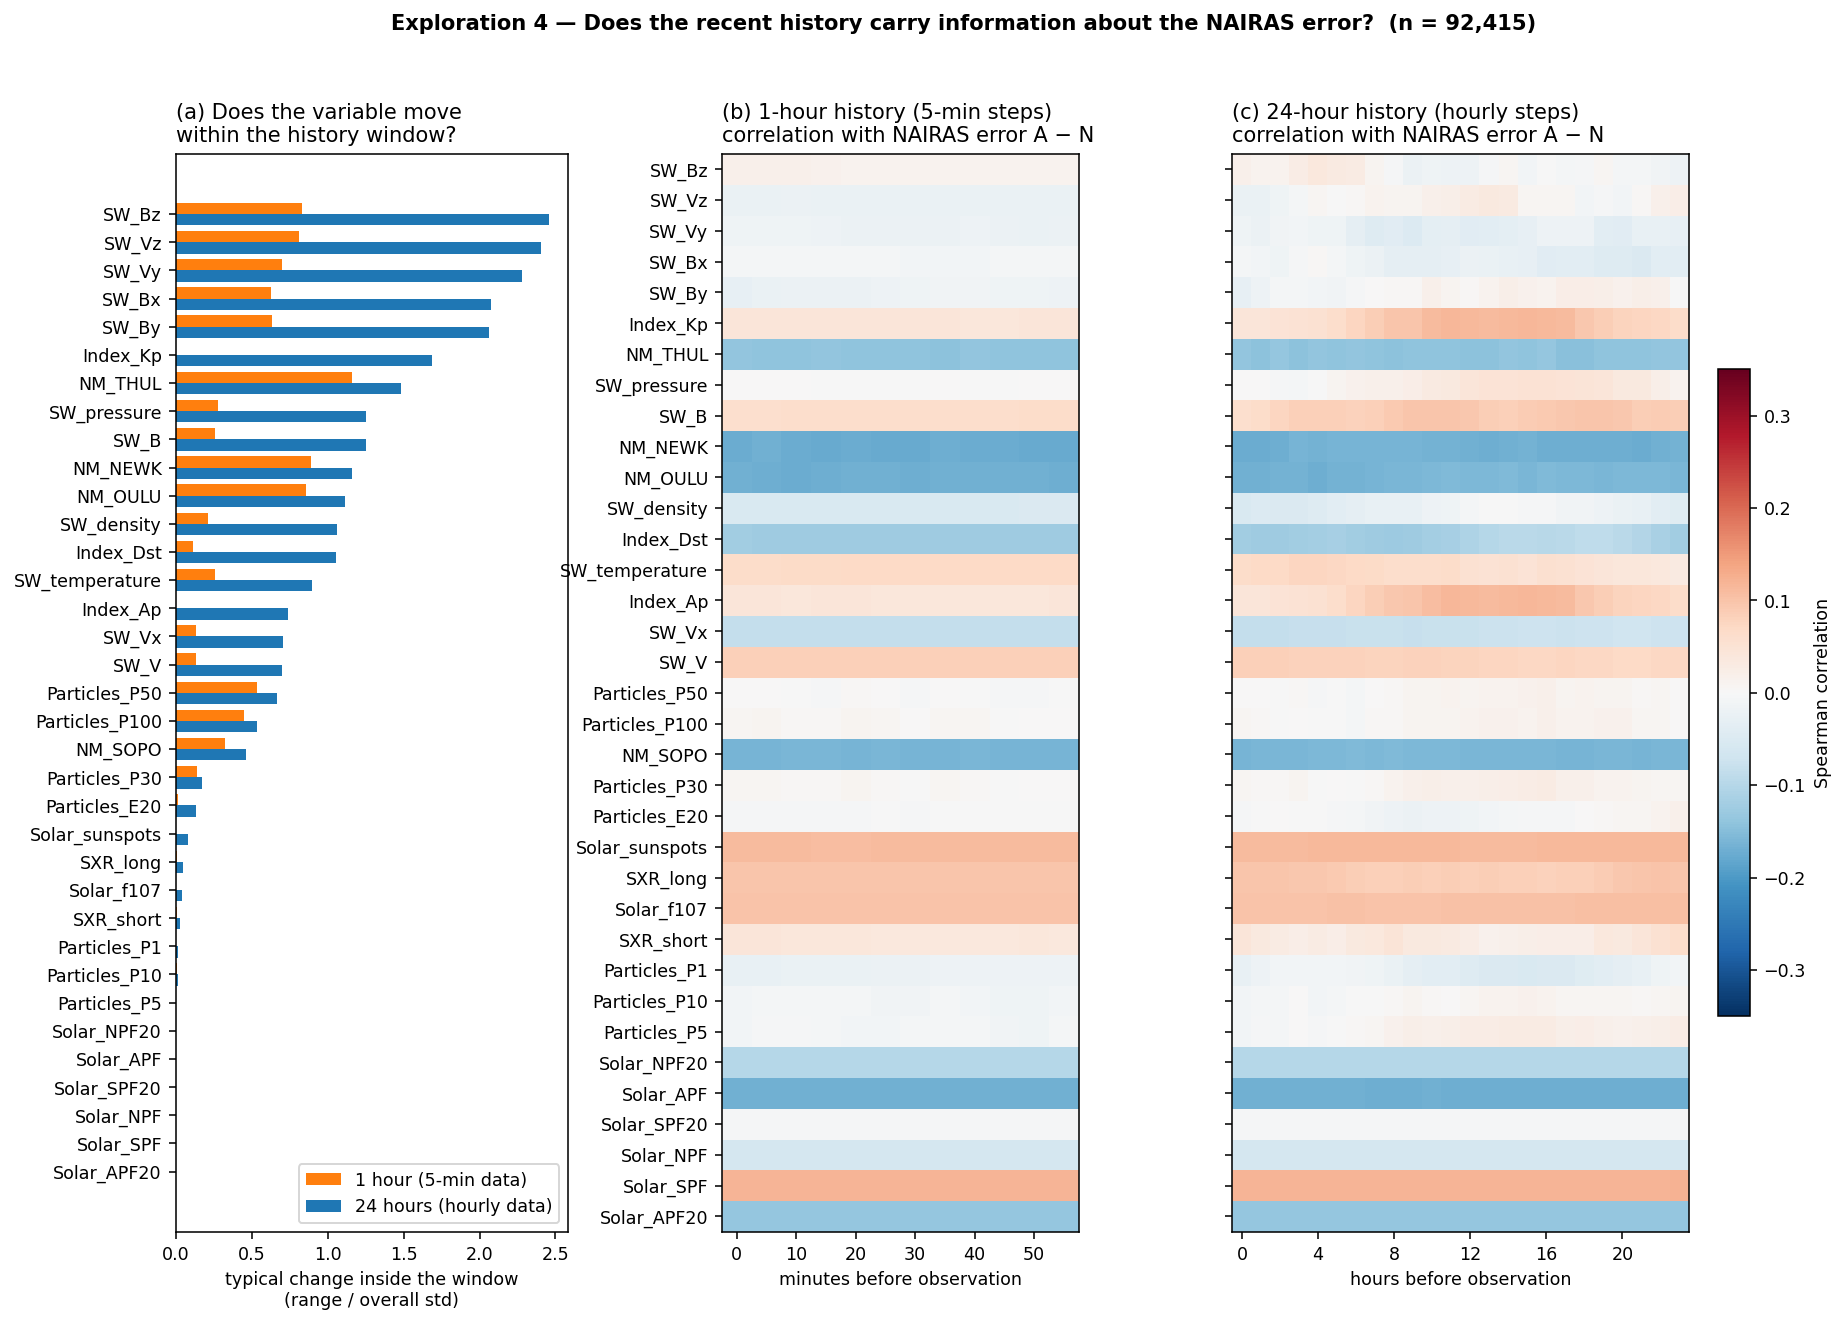
\includegraphics[width=0.95\linewidth]{e04_temporal_information.png}
\caption{Information in the environmental history for all 92,415
observations. (a) Median change of each variable inside its window (range
divided by the variable's overall standard deviation) for the 1-hour,
5-minute-cadence history (orange) and the 24-hour, hourly history (blue);
zero means the history is flat. (b, c) Spearman correlation between the
NAIRAS error $A-N$ and each variable at each lag, where column 0 is the
observation time. Horizontal stripes mean the association does not depend on
lag; Kp and Ap peak roughly 12--17~h before the observation.}
\label{fig:temporal}
\end{figure*}

\end{document}
